\documentclass{article}

\usepackage[margin=1in]{geometry}
% Names and accents 
\usepackage[T1]{fontenc}

% Math and figures
\usepackage{amsmath,amssymb}
\usepackage{graphicx}
\usepackage{float}
\usepackage{tikz-cd}
\usepackage{multicol}

\usepackage{microtype}
\usepackage{listings}
\usepackage{xcolor}
\usepackage{booktabs,array}
\usepackage{hyperref}
\usepackage{enumitem}
\usepackage{mdframed}
\usepackage{titlesec}

% Paragraphs
\setlength{\parindent}{1.5em}
\setlength{\parskip}{0pt}

% Compact academic spacing without changing the font size or margins
\titlespacing*{\section}{0pt}{2.5ex plus 0.5ex minus 0.2ex}{1ex}
\titlespacing*{\subsection}{0pt}{2ex plus 0.4ex minus 0.2ex}{0.8ex}
\titlespacing*{\subsubsection}{0pt}{1.5ex plus 0.3ex minus 0.2ex}{0.5ex}
\setlength{\textfloatsep}{10pt plus 2pt minus 2pt}
\setlength{\intextsep}{8pt plus 2pt minus 2pt}
\setlength{\abovecaptionskip}{5pt}
\setlength{\belowcaptionskip}{0pt}

% Page number
\usepackage{fancyhdr}
\usepackage{lastpage}

\usepackage{natbib}
\usepackage{url}


\bibliographystyle{plainnat}

\title{\vspace{-2.5em}Representing and Parsing Replacement Self-Repair in Formal Meaning Representations}
\author{Hongxu Zhou}

\date{}

\hypersetup{
    colorlinks=true,
    linkcolor=black,
    citecolor=black,
    urlcolor=blue
}

% Style for SBN sequences
% Save this for the thesis
% --Hongxu Zhou
\lstdefinestyle{sbn}{
    basicstyle=\ttfamily\small,
    breaklines=false,
    frame=single,
    rulecolor=\color{gray!60},
    backgroundcolor=\color{gray!6},
    xleftmargin=1.5em,
    xrightmargin=1.5em,
    framexleftmargin=1em,
    columns=flexible,
    keepspaces=true,
    showstringspaces=false,
    aboveskip=0.6em,
    belowskip=0.6em,
    commentstyle=\color{gray!80}\itshape,
    morecomment=[l]{\%},
}

\newcommand{\sbnterm}[1]{\texttt{#1}}

\begin{document}
\pagestyle{fancy}
\fancyhf{}
\fancyfoot[C]{\thepage/\pageref{LastPage}}
\renewcommand{\headrulewidth}{0pt}
\maketitle
\thispagestyle{fancy}

\section{Introduction}
\label{sec:introduction}
%============high level big picture
This interdisciplinary project brings together formal and computational semantics with natural language processing (NLP). It examines how formal meaning representations can capture replacement self-repair (RSR) in natural language.

%=============intro starts with general definition
Speakers sometimes revise an utterance before they have finished it. This
process is called self-repair, a type of disfluency with three parts
\citep{shribergPreliminariesTheorySpeech1994,
leveltMonitoringSelfrepairSpeech1983}. The \emph{reparandum} is the abandoned
material. The \emph{interregnum} is the interval between the end of the reparandum and the onset of the coming repair. It may contain an editing
expression such as \textit{I mean} \citep{clarkPausesHesitationsPsycholinguistic2006}.
The \emph{repair} is the material with which the speaker resumes the utterance.
This project focuses on replacement self-repair (RSR) within a clause, in which the
repair replaces the reparandum and changes the intended meaning.

Figure~\ref{fig:siri-repair} illustrates an RSR: 
the speaker begins by asking Siri about the weather in Berlin, then replaces
Berlin with Dublin. In the utterance, \textit{in Berlin} is the reparandum,
\textit{I mean} is the editing expression occupying the interregnum, and
\textit{in Dublin} is the repair. Although
Dublin expresses the speaker's final intention, Siri returns the weather for
Berlin.

\begin{figure}[ht]
    \centering
    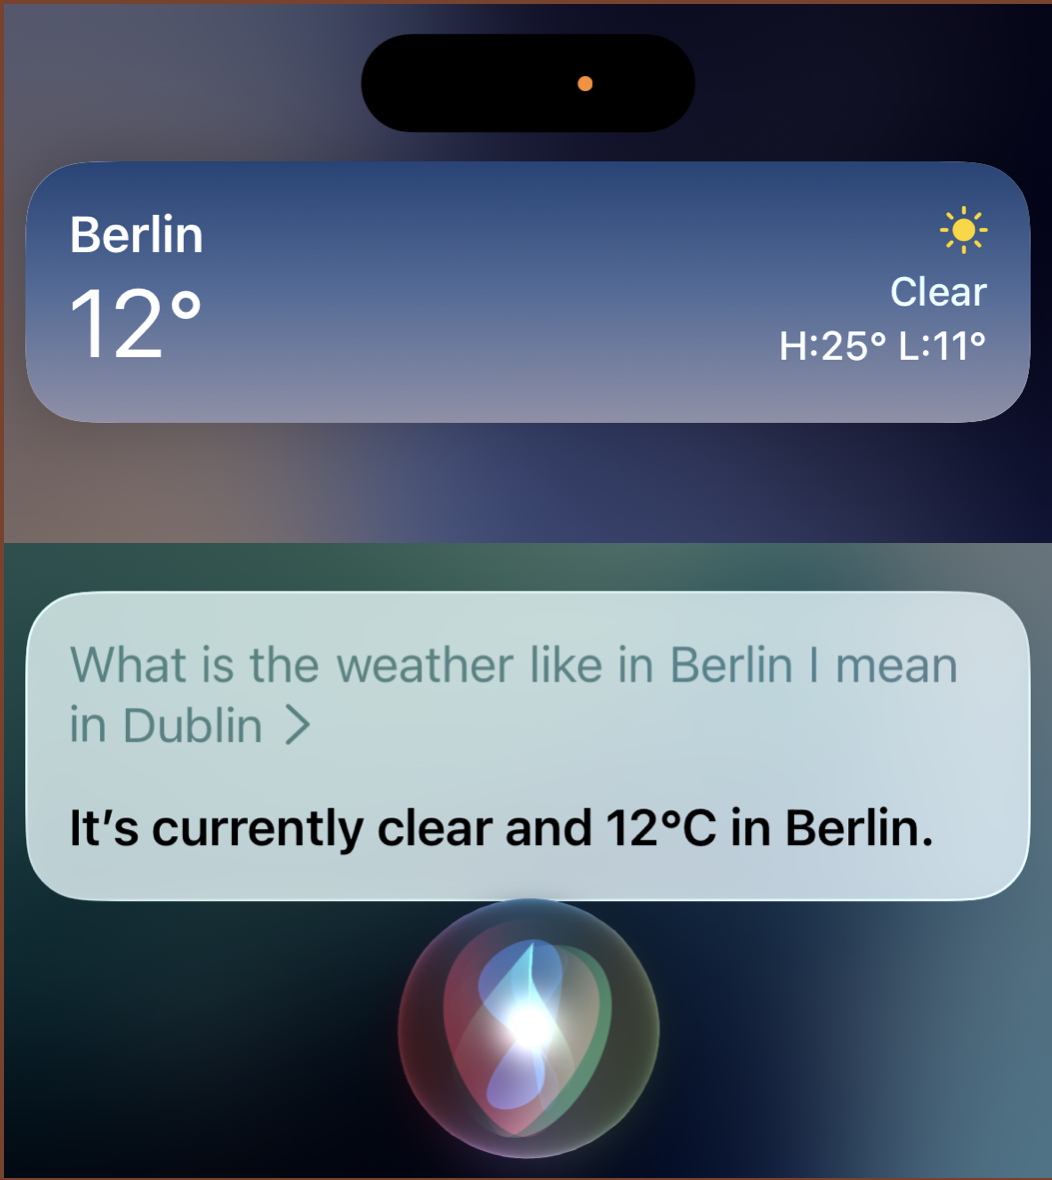
\includegraphics[width=0.45\textwidth]{viz/siri-b-i-d.png}
    \caption{Siri responds to the withdrawn location, Berlin, after the speaker
    replaces it with Dublin.}
    \label{fig:siri-repair}
\end{figure}

%=========quick LR showing previous method and limitations
Mainstream computational approaches commonly detect the reparandum and
editing expression for subsequent processing. One approach removes them while
retaining the repair, producing fluent text intended to express the speaker's
final intention \citep{johnsonTAGbasedNoisychannelModel2004}. Another retains
the spoken words and marks disfluent spans or tokens
\citep{futamiStreamingJointSpeech2023}. In the weather example, the first
approach retains only \textit{in Dublin}, while the second would preserve both cities but marks
\textit{in Berlin} as disfluent.

Explicit MRs remain useful in LLM-based systems because they make
model-interpreted meaning inspectable beyond surface text. They organise
entities, events and their relations into structures that can be examined
formally \citep{bosSequenceNotationCatching2023}. In recent work, explicit MRs
have been used to detect unsupported relations in generated database queries
\citep{reganMASSIVEMultilingualAbstract2024}, evaluate the contextual
appropriateness of dialogue responses
\citep{yangEmphasisingStructuredInformation2025} and construct
paraphrase-resistant semantic watermarks
\citep{yeSWANSemanticWatermarking2026}. These uses illustrate why explicit
semantic structure remains useful for verification, evaluation and subsequent
processing.

For applications using explicit MRs, self-repair raises the question of what
information should remain after a speaker revises an utterance.
The reparandum can continue to affect comprehension, as shown by
psycholinguistic evidence \citep{lauLingeringEffectsDisfluent2005}. It may also
remain available for later reference in dialogue
\citep{purverComputationalModelsMiscommunication2018}.

Returning to Figure~\ref{fig:siri-repair}, suppose the speaker receives the
correct response and follows with \textit{``Show me the airports of these two
cities''}, referring to both locations. Cleaned text would retain Dublin but
lose Berlin, leaving only one explicit antecedent for the plural expression
\textit{these two cities}. A transcript marked with disfluency labels would
preserve both names \citep{futamiStreamingJointSpeech2023}, but the labels would
not specify how Berlin's semantic role has been revised.

%==========turn back to my own work -- Claim
Thus, I argue that an MR for RSR should encode the semantic content of the
reparandum and repair, together with the structural configuration through which the
utterance is revised. In the running example, both cities should be linked to the weather
request, with an ordered replacement structure designating Berlin as the
withdrawn location and Dublin as the accepted one. This representation keeps
Berlin available for later reference while recording that Dublin has replaced
it in the original role. The same distinctions make a parser's output
inspectable: its errors can be traced to omitted content, incorrect status
assignments or incorrect links to shared content. The project has developed a
formal representation of within-clause RSR. The proposed thesis will validate
its coverage and train and evaluate semantic parsers that generate it.

%================WHY SBN
Simplified Box Notation (SBN)
\citep{bosQuantificationAnnotationDiscourse2021,bosSequenceNotationCatching2023}
is a suitable starting point because it combines a structured meaning
representation with a sequential format suitable for LLM generation. Its
structure can be extended to distinguish withdrawn from accepted content while
preserving their connections to the surrounding utterance. SBN is also used
for semantic annotation in the Parallel Meaning Bank (PMB), whose existing
sentence--SBN pairs provide a basis for synthesising RSR data
\citep{abzianidzeParallelMeaningBank2017}.

%=========================================RQs & Contribution

The proposed thesis will address two research questions.

\begin{enumerate}
  \item \textbf{Representation:} How should within-clause RSR
        be represented in SBN, and what are the coverage and
        limitations of the representation?
  \item \textbf{Parsing:} How well can LLM-based semantic parsers learn this
        representation from synthesised meaning-banked data, and what errors
        remain?
\end{enumerate}

This thesis aims to make three contributions.

\begin{enumerate}[itemsep=0.2em]
  \item A representation of within-clause RSR in SBN,
        together with an account of its coverage and limitations.
  \item A completed diagnostic study of how an LLM-based semantic parser
        trained on fluent sentence--SBN pairs processes RSR.
  \item A data-generation and training pipeline that constructs paired RSR
        utterances and repair-aware SBNs from meaning-banked data and trains
        LLM-based parsers to produce the repair-aware representation.
\end{enumerate}

%============Section Navigation

Section~\ref{sec:related-work} (\emph{Related Work}) reviews disfluency
processing and semantic accounts of repair. Section~\ref{sec:formalism}
(\emph{Formalism}) defines the repair-aware SBN. Section~\ref{sec:methodology}
(\emph{Methodology}) presents the diagnostic pilot, corpus construction and
model experiment. Section~\ref{sec:timeline} (\emph{Timeline}) records
completed work and remaining milestones.
\section{Related Work}
\label{sec:related-work}

The review supports two design decisions. Section~\ref{sec:rw-disfluency}
examines what NLP systems remove, preserve or recover when processing
self-repair. Section~\ref{sec:rw-representation-choice} then asks which
semantic accounts can encode the missing distinction between withdrawn and
accepted content. Readers familiar with disfluency detection may begin with
the second subsection; readers familiar with semantic representation can use
the first to locate the project's NLP task.

\subsection{Disfluency Detection and Downstream Processing}
\label{sec:rw-disfluency}

Mainstream NLP approaches use \emph{disfluency} as an umbrella term for a
range of phenomena that interrupt the fluent flow of speech, including
self-repair
\citep{shribergPreliminariesTheorySpeech1994,senSemanticParsingDisfluent2021}.
The studies reviewed below differ in their coverage of these phenomena, but
typically address them within a shared processing task. Their outputs range
from cleaned text and annotated transcripts to meaning representations for
downstream applications
\citep{johnsonTAGbasedNoisychannelModel2004,futamiStreamingJointSpeech2023,senSemanticParsingDisfluent2021}.

In a task-oriented NLP pipeline, a downstream component that books a ticket
or retrieves information typically only needs the user's final intention: which
ticket to book or which information to return. When that is the output
requirement, an upstream disfluency detector can mark material for omission
from subsequent interpretation. Recovering the user's
final intention is therefore an appropriate objective for these immediate
downstream tasks. Applied to Figure~\ref{fig:siri-repair}, however, this
objective yields a request for Dublin's weather without recording that Berlin
was first proposed and then withdrawn. The following discussion traces this
representational issue through correction models, transcript annotation and
semantic parsing from disfluent input.

Early computational models used the structural correspondences between
reparandum and repair described by \citet{leveltMonitoringSelfrepairSpeech1983}
to guide detection and correction. \citet{heemanDetectingCorrectingSpeech1994},
for example, used them to detect self-repairs as speech unfolded and identify
material to remove. Noisy-channel approaches modelled the reparandum as
material introduced into a fluent source and recovered that source for
subsequent language understanding
\citep{johnsonTAGbasedNoisychannelModel2004,honalCorrectionDisfluenciesSpontaneous2003}.
Across these approaches, structural correspondence guides the recovery of
fluent text.

Later neural methods reduced the need for hand-designed matching features.
For example, \citet{zayatsRobustCrossdomainDisfluency2018} learned similarity
patterns useful for identifying reparanda, while retaining detection as the
output task. The scope of the output labels, however, had already received
attention. \citet{zayatsMultidomainDisfluencyRepair2014} criticised the focus
on reparandum detection without type distinctions. Their model distinguished
repetitions from other types of disfluency and added labels for repair spans,
providing a richer account of self-repair in the transcript.
\citet{futamiStreamingJointSpeech2023} likewise preserved disfluent material
in joint speech recognition and disfluency detection, using either span
boundary markers or token-level fluent/disfluent labels. These approaches
preserve information that deletion would remove, with varying detail about
disfluency types and spans. Their labels do not, however, explicitly
represent how the repair replaces the reparandum's contribution to the
utterance's meaning.

An alternative is to let language models handle disfluency implicitly,
without a separate detection stage.
\citet{senSemanticParsingDisfluent2021} used a sequence-to-sequence parser
with a pre-trained RoBERTa encoder to map disfluent queries directly to
the intent-and-slot representations of their fluent counterparts. When
trained only on fluent data, it achieved 2\% exact-match accuracy on 56
disfluent queries, compared with 81\% on their fluent counterparts.
Adding targeted disfluency training data improved performance. More recent
end-to-end voice systems integrate spoken input, tool calls and spoken
responses, likewise handling disfluency without a separate detection
output. Yet in Full-Duplex-Bench-v3 \citep{linFullDuplexBenchv3BenchmarkingTool2026}, the highest task-completion rate on
scenarios containing self-repair was 58.8\%, achieved by GPT-Realtime. Reported errors include
premature commitment to tool arguments, allowing reparanda to enter
API calls. These findings indicate that reliable disfluency handling
remains a challenge across both pre-trained semantic parsers and
end-to-end voice systems.

The approaches reviewed above offer ways to detect disfluency and recover
the speaker's final intention, but leave the semantic status of withdrawn
content largely outside their output requirements. Together with the
continuing contextual role of the reparandum discussed in the introduction,
this motivates exploring alternative ways of representing self-repair.

\subsection{Formal and Computational Semantic Accounts of RSR}
\label{sec:rw-representation-choice}

This subsection compares semantic accounts of RSR and related forms of
revision, focusing on whether their representations can serve as targets for
LLM-based semantic parsing.

Dynamic Syntax with Type Theory with Records (DS-TTR) builds meaning word by
word through DS parsing actions and expresses the resulting content as TTR
record types \citep{purverIncrementalSemanticConstruction2011}.
\citet{houghProcessingSelfrepairsIncremental2012} handle RSR by
returning to an earlier parse state and continuing along a new path.
Their processing record links words, parsing actions and semantic
representations, keeping the reparandum accessible. The final accepted TTR
record type alone, however, does not identify the withdrawn path and its
replacement; that information remains in the processing history.

This project requires the final meaning representation itself to retain the
reparandum, repair and replacement structure for inspection, comparison and
scoring. DS-TTR is therefore not adopted as the basis for the target
representation because it would shift the learning and evaluation target from
a final repair-aware semantic structure to a grammar-constrained derivation.

AMR represents sentence meaning as a graph
\citep{banarescuAbstractMeaningRepresentation2013} and can be linearised for
generation by pre-trained sequence-to-sequence models
\citep{fanLeveragingAMRGraph2024}, making it a potential candidate for this project. A
close precedent comes from work on disrupted sentences.
\citet{addleseeUnderstandingDisruptedSentences2023} use underspecified AMR
graphs to represent sentences with missing content and complete them using
follow-up input. Their task recovers missing content, whereas RSR replaces
content already expressed. In Figure~\ref{fig:siri-repair}, a repair-aware
representation must therefore retain both locations and mark the status of
each.

Standard AMR nevertheless requires extension on two points. First, its
limited treatment of scope \citep{bosSquibExpressivePower2016} lacks the
separate semantic contexts needed to \emph{quarantine} the reparandum.
Its content must be retained without entering the accepted meaning. Second,
AMR abstracts away from surface word order
\citep{banarescuAbstractMeaningRepresentation2013}, so a graph and its
linearisation do not record the order of replacement updates. This order matters
because reversing which expression replaces the other changes the accepted
meaning. An AMR extension would therefore need an explicit directed relation
or a constrained linearisation. These requirements favour a context-based
framework that already separates semantic contexts and relates successive
updates.

Within such a framework, correction must distinguish the content that is
given up from the content that replaces it.
\citet{vanleusenIncompatibilityContextDiagnosis2004} characterises this
relation through contextual incompatibility. Accepting the new proposal
requires giving up the content being revised, whether that content was stated
explicitly or inferred. In Figure~\ref{fig:siri-repair}, this means withdrawing
Berlin as the location and accepting Dublin while the surrounding request
remains unchanged.

Segmented Discourse Representation Theory (SDRT)
\citep{asherLogicsConversation2003} encodes connections between discourse
units through rhetorical relations. \citet{lascaridesAgreementDisputesCommitments2009}
use \textsc{Correction} to link the corrected unit to the correcting one,
representing the incompatibility condition proposed by
\citet{vanleusenIncompatibilityContextDiagnosis2004} as the denial of prior
content and the acceptance of its correction. Their account principally concerns
corrections across conversational turns. SBN inherits this theoretical
machinery by adopting SDRT's discourse-relation inventory to connect semantic
contexts \citep{bosSequenceNotationCatching2023}. The remaining task is to
specify how the reparandum and repair connect to the shared semantic structure
of one unfinished clause. Section~\ref{sec:formalism} develops this
configuration and its interpretation.

\section{Formalism (Completed)}
\label{sec:formalism}
The proposed representation has three requirements. It must retain the
reparandum without asserting it as part of the speaker's final commitment,
identify the repair as accepted content and connect both candidates to the
structure they share. Meeting these requirements depends on SBN's treatment of
semantic roles, contexts and accessibility. Section~\ref{sec:sbn-brief}
introduces only the notation needed for this account; readers familiar with
SBN contexts and accessibility may begin with
Section~\ref{sec:paired-configuration}. Section~\ref{sec:formalism-coverage}
separates the representation's coverage from the narrower scope implemented
in the main experiment.

\subsection{SBN Requirements for the Representation}
\label{sec:sbn-brief}

SBN represents meaning as a sequence of concepts and their relations
\citep{bosSequenceNotationCatching2023}. Concepts introduce entities, events
or properties. Their labels record type and sense. In
Figure~\ref{fig:weather-rsr-comparison}(a), \sbnterm{city.n.01} introduces a
city concept and \sbnterm{Name "Dublin"} records its name. Roles connect concepts by
relative indices: \sbnterm{Location +1} points forward to the city, while
\sbnterm{Theme -1} points back to \sbnterm{weather.n.01}. Expressions such as
\sbnterm{EQU now} assign a value. The sequence therefore describes the request
without using explicit variables.

\begin{figure}[H]
\centering
\begin{minipage}[t]{0.53\textwidth}
\raggedright
\textbf{(a) No RSR}\par\smallskip
\parbox[t][3\baselineskip][t]{\linewidth}{\small\raggedright
\textit{``What is the weather like in Dublin?''}}
\begin{lstlisting}[style=sbn,
    basicstyle=\ttfamily\fontsize{7}{9}\selectfont,
    xleftmargin=0pt, xrightmargin=0pt, framexleftmargin=3pt,
    columns=fullflexible]
entity.n.01 EQU ?                                   % What
time.n.08 EQU now                                   % is
weather.n.01                                        % the weather
like.a.01 Co-Theme -3 Time -2 Theme -1 Location +1  % like 
city.n.01 Name "Dublin"                             % in Dublin?
\end{lstlisting}
\end{minipage}\hfill
\begin{minipage}[t]{0.42\textwidth}
\raggedright
\textbf{(b) Replacement self-repair}\par\smallskip
\parbox[t][3\baselineskip][t]{\linewidth}{\small\raggedright
\textit{``What is the weather like in Berlin, in Dublin?''}}
\begin{lstlisting}[style=sbn,
    basicstyle=\ttfamily\fontsize{7}{9}\selectfont,
    xleftmargin=0pt, xrightmargin=0pt, framexleftmargin=3pt,
    columns=fullflexible, escapeinside={(*@}{@*)}]
entity.n.01 EQU ?                       % What
time.n.08 EQU now                       % is
weather.n.01                            % the weather
like.a.01 Co-Theme -3 Time -2 Theme -1  % like 
    (*@\colorbox{blue!10}{\textcolor{blue!60!black}{\bfseries CORRECTION <1}}@*)
city.n.01 Name "Berlin" LocationOf -1   % in Berlin
    (*@\colorbox{blue!10}{\textcolor{blue!60!black}{\bfseries CONJUNCTION <2}}@*)                    % I mean, 
city.n.01 Name "Dublin" LocationOf -2   % in Dublin?
\end{lstlisting}
\end{minipage}
\caption{Fluent and repair-aware SBNs for the weather example. The highlighted
separators introduce the withdrawn Berlin material and the accepted Dublin
material.}
\label{fig:weather-rsr-comparison}
\end{figure}

The fluent request occupies one \emph{context}, which groups concepts with the
conditions that describe them. A \emph{separator} starts a new context when
part of the meaning requires separate interpretation. Its \emph{connector}
points to the context to which the new one relates. SBN has no closing
separator, so subsequent concepts remain in the new context until another
separator occurs or the sequence ends. For example, \sbnterm{NEGATION} places
the buying event and car in a context whose content is denied, while John
remains in the enclosing context
\citep{bosVariablefreeDiscourseRepresentation2021}:

\begin{lstlisting}[style=sbn]
male.n.02 Name "John"                  % John
    NEGATION <1                        % did not
time.n.08 TPR now
buy.v.01 Agent -2 Time -1 Theme +1     % buy
car.n.01                               % a car
\end{lstlisting}

The \sbnterm{Agent -2} link reaches out from the negated context to John. A
link in the opposite direction cannot directly reach the car introduced only
inside that context. These \emph{accessibility} restrictions determine which
concepts can be linked across context boundaries. They are central to RSR
because the reparandum must connect to shared content without becoming part of
the accepted proposition.

\subsection{The Paired RSR Configuration}
\label{sec:paired-configuration}

I propose a representation that pairs the existing separators
\sbnterm{CORRECTION} and \sbnterm{CONJUNCTION}; it introduces no new
separator.\footnote{A fuller
specification and additional examples are available at
\url{https://hongxuzhou.github.io/lct_master_project/}.} In
Figure~\ref{fig:weather-rsr-comparison}(b), \sbnterm{CORRECTION} introduces the
context containing Berlin, while \sbnterm{CONJUNCTION} introduces the context
containing Dublin. The two connectors point to the initial context containing
the shared request. Berlin and Dublin therefore occupy separate contexts with
the same parent.

The second separator is necessary because SBN does not close a context
automatically. Without it, Dublin and the continuation would remain inside
the withdrawn context. \sbnterm{CONJUNCTION} starts the accepted context and
merges its content with the shared parent
\citep{bosSequenceNotationCatching2023}. Following the treatment of corrected
content as denied in SDRT
\citep{lascaridesAgreementDisputesCommitments2009}, I give the
\sbnterm{CORRECTION} context an implicit negative interpretation. Berlin is
withdrawn; Dublin is accepted.

Both cities remain connected to the weather request. Berlin carries
\sbnterm{LocationOf -1} from the withdrawn context, and Dublin carries
\sbnterm{LocationOf -2} from the accepted context. These links identify the
role being revised. Berlin's location relation remains inside the withdrawn
content, so it does not entail that Berlin is the requested location. Dublin's
relation contributes to the accepted proposition. The representation thus
preserves the two candidates and records the change in their discourse status.

The paired configuration is realised through three constructions: the direct,
anchor and movement constructions. The direct construction requires each
candidate to carry a suitable link to shared content. A bare-subject RSR such
as \textit{``Josh, I mean, Mary
bought a cake''} lacks such a link on the subject concept itself. The
\emph{anchor construction} places a neutral \sbnterm{entity.n.01} in the shared
context and links Josh and Mary to it with \sbnterm{EQU}. The buying event
keeps one agent; Josh is withdrawn as its identification and Mary is accepted.
The PMB already uses neutral entity concepts for underspecified participants
\citep{abzianidzeParallelMeaningBank2017}. Appendix~\ref{app:devices-anchor}
gives the full construction.

A different problem occurs when the repair concept points forward to an
argument. In \textit{``Tom opened, no, broke the window''}, a copy of the
verb inside the withdrawn context cannot reach forward through both separators
to \textit{the window}. The \emph{movement construction} places the window before
the paired RSR contexts, allowing both verbs to link back to it. This preserves the
shared argument but departs from surface word order. Direct construction is
tried first. Where it fails, referential nouns can use the anchor construction,
while properties and events use the movement construction when their arguments
can be moved safely.
Appendix~\ref{app:devices} gives the listings and selection rules.

The treatment also supports later reference to accessible withdrawn
referents. Proper names can be interpreted outside the scope of negation
through presupposition
\citep[Section~7]{bosVariablefreeDiscourseRepresentation2021}. Berlin and
Dublin can therefore serve as antecedents for \textit{these two cities}, while
Berlin's location role remains withdrawn. Later reference does not restore
Berlin as the accepted location. Appendix~\ref{app:later-reference} gives the
complete \sbnterm{ANA} links. The same account does not make every item inside
a withdrawn context accessible; the challenge set is restricted to referents
for which the formal account licenses access.

Following \citet{maschlerMetalanguagingDiscourseMarkers1994},
\textit{I mean} is treated as a metalinguistic marker when it functions as an
editing expression. It is excluded from the propositional content under repair
and recorded in a \sbnterm{\%} comment on the \sbnterm{CONJUNCTION} line, as
illustrated in Figure~\ref{fig:weather-rsr-comparison}(b).

\subsection{Coverage, Implementation and Remaining Validation}
\label{sec:formalism-coverage}

The configuration can represent replacement of content expressed by SBN
concepts or roles, provided that the two candidates can connect to a shared
parent without violating accessibility. This includes replacements inside an
existing context such as negation. The corpus used in the main experiment has
a narrower implemented scope: it transforms aligned noun, verb and adjective
concepts. Role replacement is part of the representational account but is not
included in the present training data.

The paired configuration does not cover replacement of an SBN separator.
Under the current SBN rules, separators organise relations between contexts
rather than contribute content within them, so the
\sbnterm{CORRECTION}--\sbnterm{CONJUNCTION} structure cannot embed competing
separators as the reparandum and repair. Representing such cases would require
modifying SBN itself and falls outside the scope of the proposed thesis. This
limitation applies to changes in modality, such as \textit{must} to
\textit{might}, and changes in discourse relation, such as \textit{when} to
\textit{even though}, because they revise the structures that organise the
contexts. Tense and aspect replacements can also require several coordinated
concept changes and are excluded from the current corpus.

Timing sets a further boundary. The configuration covers an immediate RSR,
where the repair follows before the speaker commits intervening material.
Consider \textit{``I bought three apples from Lidl yesterday---actually,
four.''} Starting the withdrawn context at \textit{three} would also place the
location and time inside it. Moving that committed span before the context
would depart too far from the utterance order. Delayed self-repairs of this kind,
including corrections made after a completed clause, fall outside the scope of
the proposed thesis. They could be forced into the current notation only by
moving intervening committed material across contexts, at the cost of a
substantial departure from word order and SBN's preference for alignment with
the natural-language input.

The paired configuration and the direct, anchor and movement constructions
have been proposed and implemented. The completed corpus pass in
Section~\ref{sec:data} initially tests their structural applicability. The
thesis will complete the answer to the first research
question stated in Section~\ref{sec:introduction} by validating the retained corpus, examining where the constructions
succeed or fail and consolidating the resulting coverage and limitation
account. The parsing experiment then tests whether models can learn the
distinctions that the representation makes explicit.
\section{Methodology}
\label{sec:methodology}

The methodology proceeds from diagnosis to supervised testing. It begins with
a completed pilot (Section~\ref{sec:pilot}) that identifies errors in
fluent-only parsing, proceeds to corpus construction (Section~\ref{sec:data})
that converts the formal account into paired supervision, and ends with a model
experiment (Section~\ref{sec:model}) comparing normalising and repair-aware
targets.

\subsection{Pilot Study (Completed)}
\label{sec:pilot}

The completed pilot tested whether a Gemma-2 9B semantic parser
\citep{gemmateamGemma2Improving2024}, fine-tuned with LoRA only on fluent
sentence--SBN pairs \citep{huLoRALowRankAdaptation2021}, could recover the
fluent meaning from an input containing RSR. Following
\citet{senSemanticParsingDisfluent2021}, the RSR variants changed only the
natural-language input and were evaluated against the original fluent gold
SBN. Appendix~\ref{app:pilot-training}
reports the pilot training configuration.

\subsubsection{Parsing Results and Output Diagnosis}

The materials came from the English train-gold portion of PMB 5.1.0
\citep{abzianidzeParallelMeaningBank2017}. Because the source sentences and
their fluent SBN targets were included in the LoRA fine-tuning data, the parser
had been trained on the underlying fluent sentence--SBN mappings; only the
RSR-modified inputs were new. Qwen3-32B
\citep{yangQwen3TechnicalReport2025} selected a repair word and inserted a
different word of the same part of speech immediately before it as the
reparandum. The repair remained in place, keeping the intended meaning aligned
with the fluent gold SBN. After three distinct variants were generated for each source
and filtered, 833 sentences yielded 2,499 unmarked RSR inputs. Adding
\textit{I mean} between each reparandum and repair produced another 2,499.
Appendix~\ref{app:pilot-results} gives the full condition-level
results.

Each output was converted into a graph and compared with the fluent reference
SBN. The \emph{scorable rate} records how many outputs could be converted and
scored. For those outputs, SMATCH++ measures concept and relation overlap with
the reference \citep{opitzSMATCHStandardizedExtended2023}.
\emph{Failure-penalised F1} assigns zero to unscoreable outputs before averaging,
so graph-generation failures remain visible.

\begin{table}[htbp]
\centering
\small
\begin{tabular}{lrr}
\toprule
Condition & Scorable (\%) & Failure-penalised F1 \\
\midrule
Fluent      & 97.5 & 0.950$^{***}$ \\
Unmarked RSR & 94.6 & 0.786$^{***}$ \\
RSR + editing expression & 76.5 & 0.609$^{***}$ \\
\bottomrule
\end{tabular}
\caption{Parser performance across the Fluent, unmarked-RSR and
RSR-with-editing-expression input conditions. Asterisks indicate that all
three pairwise Wilcoxon signed-rank comparisons of failure-penalised F1 gave
$p<.001$.}
\label{tab:pilot}
\end{table}

Table~\ref{tab:pilot} shows a stepwise decline in both measures.
RSR lowered F1 while leaving most outputs scorable; adding \textit{I mean}
produced a further loss driven mainly by graph-generation failures. Among
outputs that remained scorable, the additional decline in F1 was much smaller.

The output patterns point to a common source of this decline. The parser often
mapped the words in the input into SBN without distinguishing their roles in
the repair. Of the 2,363 scorable RSR outputs, 90.1\% contained more concepts
than the parser's output for the corresponding fluent source sentence, with a median
of two additional concepts. Much of the fluent proposition therefore remained
recoverable, but the reparandum was often added to the asserted content rather
than interpreted as withdrawn.

Including \textit{I mean} introduced further errors into this surface-based
mapping.
Figure~\ref{fig:pilot-output} shows a parse that recovers the accepted
proposition about a cow giving birth, but also asserts the \textit{goat} and
interprets \textit{I mean} as a meaning event involving the speaker. No
structure records that the cow replaces the goat. The SBN is formally
possible, but it does not express the intended RSR.



\begin{figure}[htbp]
\centering
\small\textbf{Input:} A goat, I mean, a cow gave birth to a calf with two heads.
\par\smallskip
\begin{minipage}[t]{0.485\textwidth}
\centering
\footnotesize\textbf{Fluent reference SBN}
\begin{lstlisting}[style=sbn,basicstyle=\ttfamily\footnotesize,columns=fullflexible,breaklines=true,breakatwhitespace=true,breakindent=1em,xleftmargin=0pt,xrightmargin=0pt,framexleftmargin=2pt,framexrightmargin=2pt,aboveskip=0.25em,belowskip=0.2em]
cow.n.01    % A cow
...
\end{lstlisting}
\end{minipage}\hfill
\begin{minipage}[t]{0.485\textwidth}
\centering
\footnotesize\textbf{RSR + editing-expression parse}
\begin{lstlisting}[style=sbn,basicstyle=\ttfamily\footnotesize,columns=fullflexible,breaklines=true,breakatwhitespace=true,breakindent=1em,xleftmargin=0pt,xrightmargin=0pt,framexleftmargin=2pt,framexrightmargin=2pt,aboveskip=0.25em,belowskip=0.2em,escapeinside={(*@}{@*)}]
(*@\colorbox{yellow!30}{\strut\texttt{goat.n.01}}@*)    % A goat
(*@\colorbox{yellow!30}{\strut\texttt{person.n.01 EQU speaker}}@*)      %I
(*@\colorbox{yellow!30}{\strut\texttt{mean.v.01 Theme -2 Agent -1 Time +1}}@*)     % mean
(*@\colorbox{yellow!30}{\strut\texttt{time.n.08 EQU now}}@*)
cow.n.01    % A cow
...
\end{lstlisting}
\end{minipage}
\caption{Excerpts from the fluent reference and RSR parse. Highlighting marks
content incorrectly asserted from the reparandum and editing expression; shared
content is omitted.}
\label{fig:pilot-output}
\end{figure}

The output still receives a SMATCH++ score of 0.764 because the accepted
proposition continues to receive credit while the added content only lowers
the overlap. A substantial graph score can therefore conceal the semantic
error central to RSR. Appendix~\ref{app:pilot-goat-cow} gives the complete
RSR and fluent-input outputs.

\subsubsection{Recognition Probe and Implications}

The parsing results do not show whether the model failed to recognise RSR or
lacked an SBN pattern for representing it. I therefore removed the LoRA
adapter and asked the instruction-tuned Gemma-2 9B to mark the reparandum,
editing expression and repair in plain text. The probe detected 100.0\% of inputs
with an editing expression and 44.8\% without one, while falsely identifying RSR
in 1.0\% of fluent inputs. The editing expression was therefore a strong cue,
although detection did not ensure accurate segmentation.

The two surface forms exposed different weaknesses. Without an editing expression,
the base model missed more than half of the RSRs, while the parser often folded
both candidates into a fluent-looking graph. With \textit{I mean}, the probe
detected every RSR, but the parser often represented the expression as semantic
content. Because the probe changed both the task and the adaptation state, it
cannot isolate SBN generation as the source of error. The pilot also covered
one model size and included no repair-aware supervision. The main experiment
will therefore test repair-aware training across model sizes; the next section
describes its targets.

%==============NEW DATA SECTION
\subsection{Repair-Aware Corpus Construction}
\label{sec:data}

\subsubsection{Paired Construction}

No existing corpus pairs replacement self-repair utterances with SBN targets
that distinguish withdrawn from accepted content. The PMB contains fluent
sentence--SBN pairs \citep{abzianidzeParallelMeaningBank2017}, while speech and
disfluency resources contain self-repairs without corresponding SBN annotations
\citep{deshmukhResegmentationSWITCHBOARD1998,
passaliLARDLargescaleArtificial2022,guptaDisflQABenchmarkDataset2021}. Each PMB
source pair is therefore transformed in parallel into an RSR utterance and the
repair-aware SBN defined in Section~\ref{sec:paired-configuration}. Unlike the
pilot, which altered only the utterance, this construction changes both sides
of the pair.

Figure~\ref{fig:paired-transformation} summarises this parallel construction.

\begin{figure}[ht]
\centering
\begin{tikzcd}[column sep=8em, row sep=normal]
\text{fluent sentence} \arrow[r, "\text{insert reparandum}"] \arrow[d, "\text{PMB gold}"'] &
\text{RSR utterance} \arrow[d, dashed, "?"] \\
\text{fluent gold SBN} \arrow[r, "\text{RSR transformation}"'] &
\text{repair-aware SBN}
\end{tikzcd}
\caption{Parallel construction of an RSR utterance and repair-aware target.}
\label{fig:paired-transformation}
\end{figure}

Construction will start from a fluent sentence, its fluent gold SBN and its word--concept
alignment. An aligned noun, verb or adjective is selected as the repair, and a
different expression of the same part of speech is drawn from WordNet
\citep{millerWordNetLexicalDatabase1994} and inserted immediately before it.
For example, \textit{``She prefers tea''} becomes \textit{``She prefers
coffee, tea''}. The implemented corpus transformation replaces one aligned
lexical concept at a time; the repair follows the inserted reparandum either
immediately or after an intervening editing expression.

The repair keeps its gold representation. The transformation adds the
reparandum in the paired \sbnterm{CORRECTION} and \sbnterm{CONJUNCTION}
contexts, using the direct construction where possible and the anchor or
movement construction where required. It preserves the source graph
outside the selected replacement site. Each record stores the original and
repair-aware SBNs, the two replacement concepts, their status, their links to
shared content and the construction used. These fields pair each RSR input
with either target in the model comparison and record the information needed
to compute the structural scores in Section~\ref{sec:model}.
Appendix~\ref{app:generated-record}
shows a complete record.

\subsubsection{Validation and Selection}

Structural validation checks that the target forms a well-defined graph,
contains the paired RSR contexts, assigns withdrawn and accepted status
correctly and preserves the source graph elsewhere. It also checks the links
that connect both replacement concepts to shared content. A target that fails
any check is excluded.

A legal graph can still contain a poor training example. The competing
expressions must differ in meaning, yet both must fit the sentence context.
Bidirectional NLI scores identify replacements that remain mutually entailing
\citep{laurerLessAnnotatingMore2024}, while a causal language model measures
contextual fit as the mean token surprisal of the reparandum conditioned on
its left context. The NLI boundaries and the upper surprisal threshold are set
on a manually labelled calibration sample and frozen before the corpus is filtered. A separate sample
from the retained data estimates the proportion that satisfies both criteria.
Appendix~\ref{app:corpus-selection} gives the calibration and audit procedure.

\subsubsection{Experimental Partitions}

Every generated item inherits the train, development or test split of its PMB
source document. All variants of a source remain together, preventing a
training document from reappearing in evaluation. Every model condition also
retains the same fluent PMB component. Two training conditions receive
identical RSR utterances. The \emph{normalising} condition pairs each utterance
with its fluent gold SBN, whereas the \emph{repair-aware} condition pairs it
with the generated SBN that retains the replacement structure.

% 2026-10-24: additive recipe supersedes the original one-variant rule.
Every base RSR training item is retained without an editing expression.
An additional marked variant is constructed for approximately 30\% of base
items using one of four editing expressions---\textit{I mean}, \textit{no},
\textit{no wait} or \textit{actually}---with the same SBN target.
The current set contains 3,489 base items and 1,047 additional marked
variants, for 4,536 RSR training rows; marked variants account for 23.1\%
of these rows. Thus training retains the fluent component, adds base RSR,
and then adds marked variants. Selected items have greater row weight;
the normalising and repair-aware conditions use identical inputs and sampling.
Each test item contributes
two matched utterances with the same repair content and target.
One contains no editing expression, while the other contains one. The test
expressions include both forms seen during training and the held-out
\textit{sorry}, allowing the effect of an editing expression and
generalisation to an unseen expression to be evaluated separately.

Two test-only challenge sets contain adversarial examples that examine
behaviour that positive, sentence-local RSR examples cannot establish. The
non-RSR set contains lists, appositions and similar fluent sequences that
exhibit local surface patterns resembling RSR without expressing replacement.
It tests whether the parser distinguishes genuine repair from superficial
similarity; assigning an RSR configuration to these items counts as a false
positive. The discourse set contains controls without RSR, later reference to
the accepted referent, reference to both replacement candidates and
corrections between discourse turns. The last condition tests whether the
within-clause configuration is applied outside its scope.
Appendix~\ref{app:corpus-selection} documents selection of these cases, and
Appendix~\ref{app:later-reference} gives a complete later-reference target.

\subsubsection{Feasibility and Scope}

I have applied the implemented single-concept operator to all 9,552 English
gold documents in the PMB training partition. Table~\ref{tab:coverage-funnel}
shows the resulting structural yield before the non-RSR hold-out.

\begin{table}[ht]
\centering
\small
\begin{tabular}{@{}lrr@{}}
\toprule
Stage & Count & \% of lexical concepts \\
\midrule
Lexical concepts (noun, verb, adjective) & 23,232 & 100.0 \\
Aligned to an uttered word               & 17,886 & 77.0 \\
Usable site with a WordNet reparandum    & 16,481 & 70.9 \\
Structurally legal transformation        & 16,425 & 70.7 \\
\bottomrule
\end{tabular}
\caption{Yield of the single-concept operator over the PMB training
partition. Of the usable sites, 99.7\% produce a legal transformation.}
\label{tab:coverage-funnel}
\end{table}

The 16,425 legal transformations form the candidate pool and include the
direct, anchor and movement constructions defined in
Section~\ref{sec:paired-configuration}. Structural generation and validation are complete;
linguistic filtering, the independent audit and final sampling remain. The
sampling rule limits repeated use of a source document and is fixed before
model training.

The main corpus covers immediate replacements of aligned noun, verb and
adjective concepts. It does not include role, tense, aspect or delayed
replacements. Its WordNet-derived reparanda and written PMB contexts also
differ from spontaneous speech. The experiments will therefore test learnability
within these boundaries, not coverage of naturally occurring RSR as a whole.


%==============New Model
\subsection{Model Experiment}
\label{sec:model}

The model experiment will test whether an LLM-based semantic parser can learn
the repair-aware representation from Section~\ref{sec:data}. A parse will count
as successful only if it recovers the withdrawn and accepted content, assigns
their status and links both to the surrounding clause. The evaluation will
also test later reference, accepted meaning and generalisation beyond the
training patterns.

\subsubsection{Experimental Design}

The experiment will use instruction-tuned Qwen3.5 models at three parameter
scales: 2B, 9B and 27B \citep{qwenQwen35Native2026}. Each model size will be
trained under all three conditions, allowing the effect of the training target
to be compared across model capacities.

All conditions will retain the fluent PMB pairs (Table~\ref{tab:model-experiment}).
RSR normalisation will add the generated utterances with fluent gold SBN targets that omit
the reparandum. Repair-aware training will use the same utterances with the
repair-aware targets from Section~\ref{sec:paired-configuration}.

\begin{table}[ht]
\centering
\small
\begin{tabular}{@{}p{0.22\textwidth}p{0.16\textwidth}p{0.28\textwidth}ccc@{}}
\toprule
Training condition & RSR inputs & Target for RSR inputs & 2B & 9B & 27B \\
\midrule
Fluent only
  & No  & ---                 & $\checkmark$ & $\checkmark$ & $\checkmark$ \\
RSR normalisation
  & Yes & Fluent gold SBN    & $\checkmark$ & $\checkmark$ & $\checkmark$ \\
Repair-aware
  & Yes & Repair-aware SBN    & $\checkmark$ & $\checkmark$ & $\checkmark$ \\
\bottomrule
\end{tabular}
\caption{Training conditions and model sizes. Every model size is trained
under all three conditions with three matched random seeds. The two RSR
conditions receive the same inputs and differ in the target assigned to each
RSR item.}
\label{tab:model-experiment}
\end{table}

Within each model size, the normalising and repair-aware conditions have their
inputs, example counts and training procedure held constant, so their
comparison isolates the effect of retaining withdrawn content and its ordered
replacement structure. The fluent-only condition provides a reference without
RSR supervision, but its comparison with repair-aware training combines new
examples and new targets. Results therefore pair gains in RSR representation
with changes in accepted-meaning and fluent-input accuracy.

All conditions will use the same parsing instruction and LoRA adaptation procedure
\citep{huLoRALowRankAdaptation2021}. The instruction does not identify an input
as fluent or RSR-containing. Each model--condition combination will use three
matched random seeds, giving 27 runs in total. Outputs will be evaluated
without automatic output correction. Appendix~\ref{app:model-config}
specifies the full procedure.

\subsubsection{Evaluation}

The primary measure is \emph{RSR-structure accuracy}. An item is correct
only if its output is a well-formed graph with the paired
\sbnterm{CORRECTION}--\sbnterm{CONJUNCTION} structure. It must also assign the
reparandum and repair to the withdrawn and accepted contexts and give both the
required links to shared content. Component scores show which requirement
failed.
Graph validity and failure-penalised SMATCH++ are complementary measures
of generation success and agreement with the complete target
\citep{opitzSMATCHStandardizedExtended2023}. Appendix~\ref{app:model-metrics}
gives the metric definitions and a worked scoring example.

Two controls assess how repair-aware training affects accepted-meaning
recovery and ordinary semantic parsing. For the
automatically generated RSR items, the accepted content of each prediction is
compared with the fluent gold PMB graph after RSR-specific structure is
removed. This measures recovery of the speaker's final intention independently
of success on the reparandum. The parsers are also evaluated on the unmodified
PMB test partition. Its graph score measures ordinary semantic parsing, while
the spurious-RSR rate records fluent inputs that are incorrectly assigned RSR
structure.

The later-reference challenge set tests the main functional motivation for
retaining withdrawn material. It checks links to the accepted referent, the
withdrawn referent and both referents where the target requires them. At each
model size, the normalising and repair-aware parsers are compared because only
the latter is trained to retain the withdrawn referent and its discourse
status.

Further tests examine whether the parser has learned an RSR distinction rather
than a narrow surface pattern. Paired versions of each test item measure the
effect of an editing expression while holding its lexical content constant, and
\textit{sorry} tests a marker excluded from training. The non-RSR set
measures false alarms on lists, appositions and coordination. Cross-turn
corrections test whether the within-clause configuration is applied outside
its intended scope.

The error diagnosis distinguishes failures of RSR structure, status and
semantic-role attachment from representations of editing expressions, spurious
RSR analyses and malformed SBN. Statistical comparisons use the original PMB
source document as the unit of observation, with its variants aggregated
before testing. For each model size, the three matched seeds are compared
separately and their mean difference and range are reported; a result is
treated as stable only when its direction is consistent across seeds.
Appendix~\ref{app:model-statistics} records the full error scheme and
statistical procedure.
\section{Timeline}
\label{sec:timeline}

Table~\ref{tab:timeline} records progress and remaining work as of 23 September
2026, followed by final submission on 14 December. Each row describes one
period, with tasks in the same period proceeding in parallel where possible.

\begin{table}[ht]
\centering
\small
\setlength{\tabcolsep}{4pt}
\begin{tabular}{@{}p{0.22\textwidth}p{0.70\textwidth}@{}}
\toprule
\textbf{Period} & \textbf{Status, work and milestones} \\
\midrule
24 August--6 September
  & \textbf{Completed:} implement and run the single-concept noun, verb and
    adjective transformations; record structural coverage and blockers. \\
\addlinespace
7--20 September
  & \textbf{Completed:} structural generation and validation of the candidate
    pool. \\
\addlinespace
21 September--4 October
  & \textbf{In progress:} calibrate and freeze the linguistic filters, apply
    them to the candidate pool, prepare the independent audit sample and
    generate marker variants. Complete the two challenge sets and the
    evaluation toolkit. \\
\addlinespace
5 October--1 November
  & Run the 27 predefined Qwen3.5 adaptations and begin evaluation as
    runs finish. \\
\addlinespace
26 October--15 November
  & Complete evaluation of repair-aware parsing, editing-expression effects and
    performance on unmodified PMB data. Conduct the first error analysis by
    RSR construction.  \\
\addlinespace
16--29 November
  & Complete the error analysis and analyse the hand-written generalisation
    cases. Consolidate the representation coverage report, dataset documentation
    and experimental results in the thesis. \\
\addlinespace
30 November--6 December
  & Complete the full thesis draft and integrate the results across the
    representation, data and parsing chapters. \\
\addlinespace
7--13 December
  & Revise and proofread the thesis, check figures, tables and references, and
    prepare the submission files. \\
\addlinespace
14 December
  & Submit the final thesis. \\
\bottomrule
\end{tabular}
\caption{Project progress, remaining work and final submission schedule.}
\label{tab:timeline}
\end{table}

\clearpage
\bibliography{my_library}

\clearpage
\appendix
\section{Pilot Materials and Detailed Results}
\label{app:pilot-results}

This appendix presents the illustrative inputs, condition-level results and
representative outputs that support the pilot summary in
Section~\ref{sec:pilot}.

\subsection{Pilot Training Configuration}
\label{app:pilot-training}

The pilot parser used \texttt{google/gemma-2-9b-it} as its base model,
with LoRA fine-tuning on the fluent sentence--SBN pairs in PMB 5.1.0.
The training and development files were \texttt{train\_gold.json} and
\texttt{dev\_standard.json}, respectively. Tables~\ref{tab:pilot-lora}
and~\ref{tab:pilot-optimisation} record the training configuration used.

\begin{table}[htbp]
\centering
\small
\begin{tabular}{@{}p{0.36\textwidth}p{0.58\textwidth}@{}}
\toprule
Setting & Value \\
\midrule
Base model & \texttt{google/gemma-2-9b-it} \\
Precision & \texttt{bf16} \\
Attention implementation & \texttt{eager} \\
LoRA rank & 32 \\
LoRA scaling parameter ($\alpha$) & 64 \\
LoRA dropout & 0.05 \\
Bias adaptation & None (\texttt{bias = "none"}) \\
Target modules & \texttt{q\_proj}, \texttt{k\_proj}, \texttt{v\_proj},
  \texttt{o\_proj}, \texttt{gate\_proj}, \texttt{up\_proj},
  \texttt{down\_proj} \\
\bottomrule
\end{tabular}
\caption{Base-model and LoRA configuration. Adaptation covers both the listed
attention and MLP projections.}
\label{tab:pilot-lora}
\end{table}

\begin{table}[htbp]
\centering
\small
\begin{tabular}{@{}p{0.43\textwidth}p{0.51\textwidth}@{}}
\toprule
Setting & Value \\
\midrule
Learning rate & $2\times10^{-4}$ \\
Per-device batch size & 4 \\
Gradient accumulation steps & 4 \\
Reported effective batch size & 16 \\
Training epochs & 3.0 \\
Maximum sequence length & 1024 (updated from 512) \\
Warm-up ratio & 0.03 \\
Weight decay & 0.0 \\
Learning-rate scheduler & Cosine \\
Optimiser & \texttt{adamw\_torch} \\
Maximum gradient norm & 1.0 \\
Random seed & 42 \\
Gradient checkpointing & Enabled; \texttt{use\_reentrant = False} \\
Loss masking & Assistant SBN output only; prompt tokens excluded \\
Sequence packing & Disabled \\
Evaluation and checkpoint saving & Every 200 steps \\
Checkpoint retention limit & 3 \\
Final checkpoint selection & Load the best checkpoint by development loss
  (\texttt{eval\_loss}) \\
\bottomrule
\end{tabular}
\caption{Reported optimisation and training settings.}
\label{tab:pilot-optimisation}
\end{table}

\subsection{Input Conditions}

Table~\ref{tab:pilot-input-conditions} illustrates the fluent source sentence, three RSR
variants and their corresponding versions with an editing expression. Bold text
marks the inserted reparandum, underlined text marks the repair retained from
the source sentence, and italics mark the editing expression.

\begin{table}[ht]
\centering
\small
\begin{tabular}{@{}l>{\raggedright\arraybackslash}p{0.70\textwidth}@{}}
\toprule
\textbf{Input version} & \textbf{Example input} \\
\midrule
Fluent
  & She chatted with her friends about the baseball game. \\
RSR variant 1
  & \textbf{He}, \underline{she} chatted with her friends about the baseball
    game. \\
RSR variant 2
  & She chatted with her \textbf{coworkers}, \underline{friends} about the
    baseball game. \\
RSR variant 3
  & She chatted with her friends about the \textbf{basketball},
    \underline{baseball} game. \\
Variant 1 + editing expression
  & \textbf{He}, \textit{I mean}, \underline{she} chatted with her friends
    about the baseball game. \\
Variant 2 + editing expression
  & She chatted with her \textbf{coworkers}, \textit{I mean},
    \underline{friends} about the baseball game. \\
Variant 3 + editing expression
  & She chatted with her friends about the \textbf{basketball},
    \textit{I mean}, \underline{baseball} game. \\
\bottomrule
\end{tabular}
\caption{The seven input versions derived from one source sentence. The three
RSR variants are pooled within one condition in the main analysis; their
versions with an editing expression form the second RSR condition.}
\label{tab:pilot-input-conditions}
\end{table}

\subsection{Outcomes by Condition}

Table~\ref{tab:pilot-full} separates the two ways an output can fail to be
scored. An \emph{ill-formed} output cannot be read as SBN at all, whereas a
\emph{parse error} is produced when the sequence reads but yields an
unscoreable graph, typically through a cycle introduced by the model's own
index arithmetic.

\begin{table}[ht]
\centering
\small
\begin{tabular}{lrrrrrr}
\toprule
condition & $N$ & success \% & F1 (succ.) & F1 (failure-pen.) & ill-formed & parse error \\
\midrule
Fluent                     & 833 & 97.5 & 0.975 & 0.950 & 14 &   7 \\
\addlinespace
unmarked RSR, head         & 833 & 95.8 & 0.842 & 0.807 & 23 &  12 \\
unmarked RSR, mid          & 833 & 92.3 & 0.827 & 0.763 & 36 &  28 \\
unmarked RSR, tail         & 833 & 95.6 & 0.825 & 0.788 & 15 &  22 \\
\addlinespace
RSR + editing expression, head & 833 & 86.9 & 0.805 & 0.700 & 20 &  89 \\
RSR + editing expression, mid  & 833 & 71.8 & 0.779 & 0.559 & 30 & 205 \\
RSR + editing expression, tail & 833 & 70.7 & 0.803 & 0.568 & 14 & 230 \\
\bottomrule
\end{tabular}
\caption{Per-condition pilot results. F1 (succ.) averages over scoreable
outputs only; F1 (failure-pen.) assigns a failed output 0 and averages over all
inputs. The two rightmost columns count sentences.}
\label{tab:pilot-full}
\end{table}

The F1-among-successes and failure-penalised columns are both retained so that generation failure remains visible.

\subsection{Position Effects}

The unmarked-RSR and RSR-with-editing-expression groups are tested separately. Every sentence
appears at all three positions within its group, so the tests are paired:
Cochran's $Q$ with pairwise McNemar tests for parse success, and Friedman with
pairwise Wilcoxon tests for F1 among successes. Holm correction is applied to
the three pairwise comparisons within each group, at $\alpha = 0.05$. The F1
tests use complete triplets: 722 of 833 sentences for unmarked RSR and 408 for
the editing-expression conditions.

\begin{table}[ht]
\centering
\small
\begin{tabular}{llrlrr}
\toprule
group & outcome & $N$ & omnibus test & statistic & $p$ \\
\midrule
unmarked RSR         & parse success       & 833 & Cochran's $Q$ & 14.85 & 0.0006 \\
unmarked RSR         & F1 among successes  & 722 & Friedman      & 26.14 & $2.1\times10^{-6}$ \\
RSR + editing expression & parse success       & 833 & Cochran's $Q$ & 84.61 & $<10^{-6}$ \\
RSR + editing expression & F1 among successes  & 408 & Friedman      & 18.02 & 0.0001 \\
\bottomrule
\end{tabular}
\caption{Omnibus tests for an effect of reparandum position. All four are
significant at $\alpha = 0.05$.}
\label{tab:position-omnibus}
\end{table}

Table~\ref{tab:position-pairwise} gives the corresponding corrected pairwise
comparisons.

\begin{table}[ht]
\centering
\small
\begin{tabular}{llrrrl}
\toprule
 & & \multicolumn{3}{c}{Holm-corrected $p$} & \\
\cmidrule(lr){3-5}
group & outcome & head--mid & head--tail & mid--tail & separates \\
\midrule
unmarked RSR         & parse success      & 0.0037 & 0.897 & 0.0061 & mid (lower) \\
unmarked RSR         & F1                 & $1.9\times10^{-5}$ & $3.0\times10^{-6}$ & 0.439 & head (higher) \\
RSR + editing expression & parse success      & ${\sim}0$ & ${\sim}0$ & 0.633 & head (higher) \\
RSR + editing expression & F1                 & 0.0001 & 0.763 & 0.0005 & mid (lower) \\
\bottomrule
\end{tabular}
\caption{Pairwise position comparisons. McNemar for parse success, Wilcoxon
signed-rank for F1, Holm-corrected within each group.}
\label{tab:position-pairwise}
\end{table}

The F1 comparisons use only sentences with a scoreable output at all three
positions; this exclusion is reflected in the smaller $N$ values in
Table~\ref{tab:position-omnibus}.

\subsection{Representative Outputs}

\subsubsection{Editing-expression reification in the goat--cow example}
\label{app:pilot-goat-cow}

The example discussed in Section~\ref{sec:pilot} receives the following
output for the RSR input \textit{``A goat, I mean, a cow gave birth to a calf
with two heads''}:

\begin{lstlisting}[style=sbn]
% SPURIOUS: editing-expression material reified as content
goat.n.01                                    % goat
person.n.01 EQU speaker                      % I
mean.v.01 Theme -2 Agent -1 Time +1          % mean
time.n.08 EQU now
% GOLD-EQUIVALENT: the actual proposition
cow.n.01                                     % cow
give_birth.v.01 Agent -1 Time +1 Patient +2  % gave birth
time.n.08 TPR now                            % gave
calf.n.01 Part +2                            % calf
quantity.n.01 EQU 2                          % two
head.n.01 Quantity -1                        % heads
\end{lstlisting}

For comparison, the parser produces the following gold-equivalent output for
the fluent input \textit{``A cow gave birth to a calf with two heads''}:

\begin{lstlisting}[style=sbn]
cow.n.01                                     % cow
give_birth.v.01 Agent -1 Time +1 Patient +2  % gave birth
time.n.08 TPR now
calf.n.01 Part +2                            % calf
quantity.n.01 EQU 2                          % two
head.n.01 Quantity -1                        % heads
\end{lstlisting}

\subsubsection{Retention and loss of replacement candidates}

The following outputs document two error patterns behind the aggregate scores.
They are drawn from a purposive sample and are not used to estimate error
frequency. Both come from \textit{p07/d1400}, whose gold sentence is
\textit{``Is it true that you are in love with me?''} and whose fluent-input parse the
model recovers exactly:

\begin{lstlisting}[style=sbn]
time.n.08 EQU now
entity.n.01
true.a.01 Time -2 Proposition >1 EQU -1
    CONTINUATION <0
person.n.01 EQU hearer                        % you
time.n.08 EQU now
in_love.a.01 Experiencer -2 Time -1 Stimulus +1
person.n.01 EQU speaker                       % me
\end{lstlisting}

For the uncued input \textit{``Is it true that I am, you are in love with
me?''}, both candidates remain in the output:

\begin{lstlisting}[style=sbn]
% ... as above, up to the CONTINUATION
person.n.01 EQU speaker
time.n.08 EQU now
in_love.a.01 Experiencer -2 Time -1 Stimulus +1
person.n.01 EQU hearer
    CONTINUATION <1                           % the reparandum reading, retained
person.n.01 EQU hearer
time.n.08 EQU now
in_love.a.01 Experiencer -2 Time -1 Stimulus +1
person.n.01 EQU speaker
\end{lstlisting}

The output scores 0.743 against the fluent reference graph. When
\textit{``I mean''} is inserted, the output retains only the reparandum reading
and scores 0.926:

\begin{lstlisting}[style=sbn]
time.n.08 EQU now
entity.n.01
true.a.01 Time -2 Proposition >1 EQU -1
    CONTINUATION <0
person.n.01 EQU speaker                       % "I", the withdrawn candidate
time.n.08 EQU now
in_love.a.01 Experiencer -2 Time -1 Stimulus +1
person.n.01 EQU hearer                        % "me", now resolved to the hearer
\end{lstlisting}

These examples supplement the shorter output shown in
Section~\ref{sec:pilot}. Together, they show that high graph overlap can
coexist with retention of asserted reparandum material or loss of the accepted
repair.

\subsection{Recognition Probe Results}

That the parser fails to represent the RSR does not show the RSR was
invisible to it. A separate probe put the question to the base model, without
the adapter, which was asked to mark the reparandum, editing expression and repair in
plain text. Span scores are computed over sentences that were detected and
carry a true RSR.

\begin{table}[ht]
\centering
\small
\begin{tabular}{lrrrrrr}
\toprule
condition & $N$ & detected \% & off-template \% & scored & reparandum F1 & repair F1 \\
\midrule
unmarked RSR, head          & 833 & 30.7 &  0.0 & 254 & 0.667 & 0.487 \\
unmarked RSR, mid           & 833 & 39.0 &  0.0 & 324 & 0.503 & 0.420 \\
unmarked RSR, tail          & 833 & 64.2 &  0.7 & 536 & 0.489 & 0.340 \\
\addlinespace
RSR + editing expression, head & 833 & 100.0 &  0.6 & 831 & 0.900 & 0.862 \\
RSR + editing expression, mid  & 833 & 100.0 &  4.9 & 832 & 0.822 & 0.775 \\
RSR + editing expression, tail & 833 & 100.0 & 19.3 & 831 & 0.627 & 0.662 \\
\bottomrule
\end{tabular}
\caption{Base-model detection of self-repair in plain text. Off-template counts
outputs that did not follow the requested response format.}
\label{tab:ablation}
\end{table}

These figures report the condition-level values summarised in
Section~\ref{sec:pilot}. Detection rate and span F1 are reported separately
because identifying the presence of an RSR does not guarantee correct
segmentation of its components.

\section{Corpus Selection and Audit}
\label{app:corpus-selection}

This appendix records how structurally legal candidates are filtered and
sampled before model training. All boundaries and sampling decisions are
frozen before any main-experiment test output is inspected.

\subsection{Linguistic Calibration}

A 200-item calibration sample is drawn from the structurally legal pool,
stratified by noun, verb and adjective replacements and by the available
direct, anchor and movement constructions. Each item receives separate binary
judgements for semantic contrast and contextual plausibility. A replacement
such as \textit{``couch, I mean, sofa''} lacks sufficient contrast, whereas
\textit{``cake, I mean, carburettor, for his wedding''} lacks contextual
plausibility despite the lexical contrast.

Bidirectional NLI scores are calibrated against the contrast judgements, and
the mean token surprisal of the reparandum conditioned on its left context is
calibrated against the plausibility judgements. Each boundary, including the
upper surprisal threshold, is selected on the calibration sample and then held
fixed for the full candidate pool. Items that fail either criterion are
removed. After filtering, a separate 200-item sample receives the same manual
judgements. Its results estimate the retained corpus's rates of semantic
contrast, contextual plausibility and joint validity; this audit sample does
not alter the thresholds.

\subsection{Sampling and Split Audit}

All generated variants retain the PMB split and document identifier of their
source. A split audit verifies that no identifier occurs in more than one of
the training, development and test partitions. The final sample contains at
most two replacement sites from one source document. Where a document contains more
eligible sites, selection uses a fixed random seed and is stratified by part
of speech and construction. The realised corpus counts are frozen
before training and shared by the normalising and repair-aware conditions.

% 2026-10-24: preserve all base forms and append selected marked variants.
Every unmarked base form is retained. Marked variants are appended for
1,047 base items (30\%, rounded), including all 482 items flagged as
potentially ambiguous without a marker. The remaining 565 are sampled
proportionally to the non-ambiguous pool sizes by repair type, using largest
remainders and seed 20261024. Marker assignment uses seed 20261025 and
balances the four expressions within each type and across the selected set.
Ambiguity flags are heuristic; retaining the unmarked forms leaves textual
ambiguity as a limitation. Each surface variant has a unique identifier
and retains its base-item and source-document identifiers.
Test
sites retain their paired marked and unmarked forms under the same source
identifier, allowing them to be aggregated before statistical comparison.

\subsection{Challenge-Set Selection}

The non-RSR hold-out begins with 105 candidate PMB training documents,
which are removed from both the fluent training component and the RSR source
pool before fine-tuning. This leaves 9,447 PMB training documents. Manual
screening retains lists, appositions and coordination structures that resemble
the generated RSR surface pattern but carry no replacement reading. Comparable
items from the standard PMB test partition are added without changing their
fluent gold SBNs.

The discourse challenge set is assembled after the main sentence-level data
are frozen. Selected PMB documents and hand-written cases cover fluent
multi-sentence controls, later reference to accepted content, reference to
both replacement candidates and correction between discourse turns. Only
referents licensed as accessible by Section~\ref{sec:paired-configuration} are
used in targets that refer back to withdrawn content.

\section{Model and Evaluation Specifications}
\label{app:model-evaluation}

This appendix records the implementation and scoring decisions for the model
experiment in Section~\ref{sec:model}. The main text states the
comparisons and the evidence needed to answer the research question; the
details below make those decisions reproducible.

\subsection{Model Configurations and Run Matrix}
\label{app:model-config}

Each of the 2B, 9B and 27B models receives three matched-seed runs under each
condition: fluent only, RSR normalisation and repair-aware. The full design
therefore contains 27 runs. Matching seed values across conditions within each
model size reduces avoidable variation in the normalising--repair-aware
comparison.

Every run uses the same parsing instruction and LoRA adaptation method. The
prompt asks for an SBN sequence but does not label the input as fluent or
RSR-containing. Within each model size, the fluent data, RSR inputs, training steps
and optimisation settings are held constant wherever the conditions permit.
The development checkpoint with the lowest development loss is selected
without consulting test outputs. The final experiment record will include the
model checkpoint, prompt, LoRA targets, rank and scaling, optimiser settings,
batch construction, sequence limit, seed and selected checkpoint for every
run.

\subsection{Repair-Aware Evaluation Metrics}
\label{app:model-metrics}

RSR-structure accuracy is a binary score for each generated RSR item. A
prediction receives one point only when all four requirements hold:

\begin{enumerate}[nosep]
  \item the SBN sequence can be converted into a well-formed graph;
  \item the output contains the paired \sbnterm{CORRECTION} and
        \sbnterm{CONJUNCTION} contexts required by the target;
  \item the target reparandum is in the withdrawn context and the target repair
        is in the accepted context; and
  \item both parts have the semantic-role links to shared content required by
        the gold graph.
\end{enumerate}

The four requirements are also reported separately. These component scores
distinguish a missing configuration from reversed status or incorrect
attachment. Failure-penalised SMATCH++ assigns zero to an output that cannot be
scored and otherwise measures overlap with the complete repair-aware graph.
Results grouped by the direct, anchor and movement constructions show whether
the construction used affects parsing difficulty.

Accepted-meaning evaluation projects a prediction onto the speaker's final
meaning. The withdrawn context and the RSR-specific operators are removed, while
the accepted content and the surrounding graph are retained. The projected
graph is compared with the fluent gold PMB graph. On the unmodified PMB
test partition, the evaluation reports failure-penalised SMATCH++, graph
validity and the proportion of outputs that introduce an RSR configuration.

\subsection{Worked Scoring Example}
\label{app:model-scoring}

Consider \textit{``Let's stand, I mean, sit in the shade''}. The target marks
\textit{stand} as withdrawn and \textit{sit} as accepted, with both events
connected to the shared participants and time. An output that places both
verbs in ordinary asserted content may retain much of the target graph and
receive partial SMATCH++ credit. Its RSR-structure accuracy is nevertheless
zero because it does not express the replacement. An output receives full
RSR-structure credit only when the contexts, status assignments and shared
links are all correct. Removing its withdrawn context should then yield the
fluent meaning of \textit{``Let's sit in the shade''} for accepted-meaning
evaluation.

\subsection{Error Annotation Guidelines}
\label{app:model-errors}

The diagnostic categories are fixed before the main test outputs are
inspected. They distinguish a missing RSR configuration, reversed
withdrawn and accepted status, an incorrect link to shared content, a
reparandum left in accepted content, an editing expression represented as ordinary
semantic content, a spurious RSR analysis on fluent input and malformed SBN. Categories
may co-occur when they describe separate faults in one output. Any pattern
first identified from the main test outputs will be reported as a post-hoc
observation and excluded from the planned comparison.

\subsection{Statistical Comparisons}
\label{app:model-statistics}

All variants derived from one PMB source document are averaged before a
comparison, making the source document the unit of observation. For each model
size and matched seed, paired document-level differences are reported with
95\% confidence intervals from 10,000 paired bootstrap samples. Within each
model size, the mean and range of the three seed-specific differences
summarise training variation. A result is interpreted as stable only when all
three differences have the same direction. Holm correction is applied within
each family of secondary comparisons.

\section{A Later-Reference Challenge Example}
\label{app:later-reference}

The following hand-written target extends the Berlin--Dublin replacement from
the introduction with a second utterance that refers to both cities. It
illustrates the type of later-reference case reserved for the test-only
challenge set in Section~\ref{sec:data}.

\begin{lstlisting}[style=sbn]
% Utterance 1: What's the weather like in Berlin, I mean, in Dublin?
entity.n.01 EQU ?                              % what
be.v.01 Theme -1 Time +1 Co-Theme +2           % 's ... like
time.n.08 EQU now
weather.n.01                                   % the weather
    CORRECTION <1
city.n.01 Name "Berlin" LocationOf -1          % [reparandum] in Berlin
    CONJUNCTION <2                             % I mean,
city.n.01 Name "Dublin" LocationOf -2          % [repair] in Dublin
% Utterance 2: Show me the airports of these two cities.
    CONTINUATION <1
person.n.01 EQU hearer                         % imperative addressee
show.v.04 Agent -1 Recipient +1 Theme +2       % show
person.n.01 EQU speaker                        % me
airport.n.01 Location +2                       % the airports of
quantity.n.01 EQU 2                            % two
city.n.01 ANA -7 ANA -6 Quantity -1            % these ... cities
\end{lstlisting}

Here, \sbnterm{CONTINUATION <1} opens the context for the second
utterance and links it to the accepted context. The two
\sbnterm{ANA} links encode Berlin and Dublin as the intended plural
antecedent. This hand-written target operationalises the challenge case.

\section{RSR Constructions and Transformation Coverage}
\label{app:devices}

This appendix details the three constructions introduced in
Section~\ref{sec:paired-configuration}, states which one applies to a given
site, and reports the coverage of the concept-replacement operator over the PMB
training partition.

\subsection{The anchor construction}
\label{app:devices-anchor}

The paired configuration attaches both replacement candidates to the content
they share. Where the reparandum carries a role of its own, as
\sbnterm{Berlin} does in Figure~\ref{fig:weather-rsr-comparison}(b), that role
does the work. A subject concept selected as the repair has no such role. Taking \textit{``Josh
bought a cake''} as the source,

\begin{lstlisting}[style=sbn]
male.n.02 Name "Josh"                  % Josh
time.n.08 TPR now                      % (past)
buy.v.01 Agent -2 Time -1 Theme +1     % bought
cake.n.01                              % a cake
\end{lstlisting}

\noindent moving \sbnterm{male.n.02} into a \sbnterm{CORRECTION} context would
leave it with no link at all, since its only connection to the sequence is the
\sbnterm{Agent} role that the buying event points at it. The anchor construction inserts
a neutral \sbnterm{entity.n.01} concept before the \sbnterm{CORRECTION},
redirects the inbound role onto it, and attaches both candidates with
\sbnterm{EQU}:

\begin{lstlisting}[style=sbn]
entity.n.01                            % (anchor)
    CORRECTION <1
male.n.02 Name "Josh" EQU -1           % Josh
    CONJUNCTION <2
female.n.02 Name "Mary" EQU -2         % I mean, Mary
time.n.08 TPR now
buy.v.01 Agent -4 Time -1 Theme +1     % bought
cake.n.01                              % a cake
\end{lstlisting}

The buying event now takes the anchor as its \sbnterm{Agent}, and the two
candidates each assert an identity with it from inside their own context. The
withdrawn content is the identification of that individual as Josh, and the
accepted content is the identification as Mary. Neither \sbnterm{EQU} link
crosses a boundary in a forbidden direction, since both are negative indices
reaching outward to a concept in the parent context.

\subsection{The movement construction}
\label{app:devices-movement}

A positive index may not cross from a \sbnterm{CORRECTION} context into the
repair that follows it, which creates a problem whenever the repair concept
points forward. In \textit{``Tom broke the window''},

\begin{lstlisting}[style=sbn]
male.n.02 Name "Tom"                   % Tom
time.n.08 TPR now                      % (past)
break.v.01 Agent -2 Time -1 Theme +1   % broke
window.n.01                            % the window
\end{lstlisting}

\noindent a reparandum copy of \sbnterm{break.v.01} placed before the
\sbnterm{CORRECTION} would need \sbnterm{Theme +1} to reach
\sbnterm{window.n.01}, and that index would run through both separators. The
window is moved in front of the \sbnterm{CORRECTION} instead, so that both
copies reach it backwards:

\begin{lstlisting}[style=sbn]
male.n.02 Name "Tom"                   % Tom
time.n.08 TPR now
window.n.01                            % (moved from the end)
    CORRECTION <1
open.v.01 Agent -3 Time -2 Theme -1    % opened
    CONJUNCTION <2
break.v.01 Agent -4 Time -3 Theme -2   % I mean, broke
\end{lstlisting}

The movement construction changes the order of the representation:
\textit{the window} is uttered last but represented third. This is the
departure from word order noted in
Section~\ref{sec:formalism-coverage}, and it is accepted because the
alternative is to quarantine material the speaker kept. The move is confined to
arguments of the repair concept itself. Material that was uttered and
committed between the reparandum and the repair, as in the Lidl example, would
have to be carried past both separators, and that case is left outside the
configuration.

\subsection{Which construction applies}
\label{app:devices-order}

The direct construction is tried first at every site, since it changes neither
the inventory of concepts nor their order. Where it fails, the choice between
the anchor and movement constructions follows from the type of the repair
concept. The anchor construction asserts
\sbnterm{entity.n.01 EQU}~$c$ for each candidate $c$, which reads correctly
only when $c$ denotes a referent. Equating an entity with a property or an
event is not what the subject-RSR case supports, so for adjectives, adverbs
and verbs the movement construction is tried before the anchor, even though it
costs surface order. For nouns the order is reversed.
Table~\ref{tab:devices-coverage} shows the resulting distribution. Nouns take
the anchor construction at about the rate they take the direct construction,
while nearly all of the movement cases are adjectives.

\subsection{Coverage by part of speech}
\label{app:devices-coverage}

Table~\ref{tab:devices-coverage} breaks down the funnel of
Table~\ref{tab:coverage-funnel} by the part of speech of the repair concept
and by the construction the site ended up needing.

\begin{table}[ht]
\centering
\small
\begin{tabular}{@{}lrrrrrrr@{}}
\toprule
& & & & & \multicolumn{3}{c}{Construction used} \\
\cmidrule(l){6-8}
POS & Lexical & Aligned & Usable & Legal & Direct & Anchor & Movement \\
\midrule
Noun      & 11,781 & 10,060 & 9,560 & 9,525 & 4,576 & 4,949 &   0 \\
Verb      &  8,609 &  5,091 & 4,229 & 4,221 & 4,170 &     7 &  44 \\
Adjective &  2,842 &  2,735 & 2,692 & 2,679 & 2,050 &   148 & 481 \\
\midrule
Total     & 23,232 & 17,886 & 16,481 & 16,425 & 10,796 & 5,104 & 525 \\
\bottomrule
\end{tabular}
\caption{Candidate sites and transformation outcomes over the 9,552 English
gold documents of the PMB training partition. \emph{Aligned} counts concepts
that can be tied to an uttered word, \emph{usable} those for which WordNet
contains an eligible reparandum candidate, and \emph{legal} those where the transformation produces a
well-formed graph.}
\label{tab:devices-coverage}
\end{table}

Two of the drops deserve comment. Some 23\% of lexical concepts cannot be
aligned to an uttered word, and verbs account for most of that loss; a concept
with no surface expression cannot be given a competing expression either. A
further 6\% survive alignment but have no WordNet reparandum available, which
mainly affects senses with no co-hyponyms of the right part of speech.

\subsection{Why transformations fail}
\label{app:devices-blockers}

Of the 16,481 usable sites, 56 produce no legal graph under any of the three
options. Three conditions account for them, and they overlap, since a site may
be rejected differently by each option tried:

\begin{itemize}[nosep]
  \item \textbf{Index overflow} (45 sites). The PMB's released index pattern
    matches a single digit, so a role index may not exceed nine positions in
    either direction. Inserting two contexts pushes some existing indices past
    that ceiling. The limit belongs to the released tooling rather than to the
    notation, and it would disappear if the pattern were widened.
  \item \textbf{No attachment for the reparandum} (23 sites). Neither the
    original role nor the anchor construction leaves the withdrawn concept
    connected to the rest of the graph.
  \item \textbf{Movement unavailable} (50 sites). The repair concept has
    forward arguments that cannot be brought in front of the
    \sbnterm{CORRECTION} without moving material that belongs elsewhere.
\end{itemize}

Two further checks, for cycles and for collisions between the inserted
separators and those already present, reject individual attempts rather than
whole sites. Every site that triggered one was rescued by another option, so
neither appears in the tally above.

\subsection{Example Generated Corpus Record}
\label{app:generated-record}

Table~\ref{tab:worked-record} shows the complete record stored for one
generated replacement. The fields retain the PMB source, the choices made by
the transformation operator, both surface forms, the repair-aware SBN and the
outputs used for structural and linguistic validation. They are grouped by
function so that the generated training pair can be read separately from the
metadata retained for tracing and filtering it.

\begin{table}[ht]
\centering
\small
\begin{tabular}{@{}lp{0.62\textwidth}@{}}
\toprule
Field & Value \\
\midrule
\multicolumn{2}{@{}l}{\textit{PMB source}} \\
\addlinespace[0.25em]
\texttt{doc\_id}             & \texttt{p42/d1468} \\
\texttt{split}               & \texttt{train} \\
\texttt{nl\_clean}           & Let's sit in the shade. \\
\texttt{sbn\_clean}          & \texttt{time.n.08 TSU now person.n.01 EQU speaker sit.v.01 Time -2 Theme -1 Location +1 shade.n.01} \\
\midrule
\multicolumn{2}{@{}l}{\textit{Repair selection and transformation}} \\
\addlinespace[0.25em]
\texttt{concept\_pos}        & \texttt{2} (the repair concept is the third in
                               the sequence; positions are counted from zero) \\
\texttt{repair\_synset}      & \texttt{sit.v.01} \\
\texttt{reparandum\_synset}  & \texttt{stand.v.01} \\
\texttt{reparandum\_surface} & stand \\
\texttt{strategy}            & \texttt{inplace} \\
\texttt{devices}             & \texttt{d1\_drop\_role} \\
\texttt{blockers}            & --- \\
\texttt{max\_abs\_index}     & \texttt{3} (the largest role index in the output,
                               taken without its sign; the ceiling is nine) \\
\midrule
\multicolumn{2}{@{}l}{\textit{Generated pair}} \\
\addlinespace[0.25em]
\texttt{nl\_repair}          & Let's stand, sit in the shade. \\
\texttt{nl\_repair\_interr}  & Let's stand, I mean, sit in the shade. \\
\texttt{sbn\_repair}         & \texttt{time.n.08 TSU now person.n.01 EQU speaker CORRECTION <1 stand.v.01 Time -2 Theme -1 CONJUNCTION <2 sit.v.01 Time -3 Theme -2 Location +1 shade.n.01} \\
\midrule
\multicolumn{2}{@{}l}{\textit{Validation and filtering}} \\
\addlinespace[0.25em]
\texttt{legal}               & \texttt{1}, meaning the transformation produced a
                               well-formed graph. Items recorded as \texttt{0}
                               are dropped before any further filtering \\
\texttt{entail\_fwd}         & 0.0005 \\
\texttt{entail\_bwd}         & 0.0005 \\
\texttt{synonymy}            & 0.0005 \\
\bottomrule
\end{tabular}
\caption{A complete record produced by the current corpus-construction
pipeline. The ceiling on \texttt{max\_abs\_index} is the single-digit index
pattern described in Appendix~\ref{app:devices-blockers}; a transformation
that exceeds it is recorded as \texttt{legal 0} with
\texttt{index\_overflow} among its blockers.}
\label{tab:worked-record}
\end{table}

\end{document}
